\documentclass[12pt, a4paper]{article}

\usepackage[utf8]{inputenc}
\usepackage{amsmath}
\usepackage{graphicx}
\usepackage{geometry}
\usepackage{caption}
\usepackage{subcaption}
\usepackage{float}
\usepackage{cite}
\usepackage{hyperref}

\geometry{top=1in, bottom=1in, left=1in, right=1in}

\title{\textbf{Design of a Multi-Stage Digital Decimation Filter for Sigma-Delta ADCs}}
\author{
    Priyanandan S (B231179EE) \\
    Robin John (B231205EE) \\
    Sanad Bin Sayed (B231220EE)
}
\date{\today}

\begin{document}

\maketitle

\begin{abstract}
This paper presents the design, implementation, and verification of a multi-stage digital decimation filter for use in oversampled Sigma-Delta Analog-to-Digital Converters (ADCs). The digital decimation filter is an important part of the Sigma-Delta ADC and is designed to make the system meet high performance requirements, typically targeting a Signal-to-Noise Ratio (SNR) of not less than 120 dB and an Equivalent Number of Bits (ENOB) of not less than 20 bits. It adopts a three-stages cascaded structure including a Cascaded Integrator Comb (CIC) decimation filter, a Finite Impulse Response (FIR) compensation filter, and a half-band (HB) filter. This specific structure effectively reduces the required multiplier and memory cells by about 13\%. The system is implemented in Verilog utilizing fixed-point Q15 arithmetic and structural optimizations, and verified using a Cocotb testbench against simulated analog non-idealities.
\end{abstract}

\textbf{Keywords:} Sigma-Delta ADC, CIC Filter, Compensation FIR, Half-band FIR, Decimation, Noise Shaping, Fixed-Point Arithmetic.

\tableofcontents
\newpage

\section{Introduction}
As digital information technology develops rapidly, the precision of signal processing in medical, aerospace, and other fields requires continuous improvement. Sigma-Delta ADCs have become the architecture of choice for high-resolution applications due to their characteristics of low power consumption, high accuracy, and high linearity. 

Due to the limitations of chip technology, the conversion accuracy of traditional ADCs (like successive approximation or parallel comparison ADCs) has reached a bottleneck. The Sigma-Delta ADC can conquer these limitations by utilizing over-sampling and noise shaping technology, which dramatically improves ADC accuracy and performance. To achieve this, the architecture relies heavily on a robust digital back-end to filter the out-of-band quantization noise and downsample the signal. This paper details our three-stage digital filtering approach, including our structural optimizations and Verilog implementation pipeline.

\section{Sigma-Delta ADC Architecture}
A standard Sigma-Delta ADC is composed of a Sigma-Delta modulator and a digital decimation filter. The accuracy is mainly determined by the modulator, while the area and power consumption are mainly determined by the digital decimation filter.

\begin{figure}[H]
    \centering
    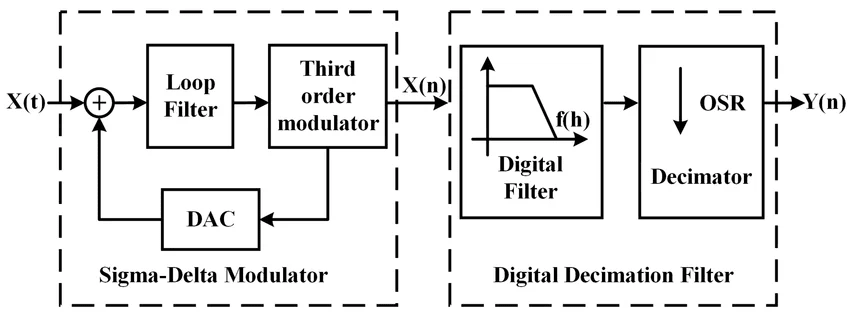
\includegraphics[width=0.8\textwidth]{Block-diagram-of-the-Sigma-Delta-ADC.png}
    \caption{General Block Diagram of a Sigma-Delta ADC}
    \label{fig:sd_adc}
\end{figure}

\subsection{Analog Sigma-Delta Modulator}
The analog front-end modulates analog signals into high-speed, low resolution oversampled signals, pushes quantization noise to high frequency, and thus achieves high SNR and ENOB. Assuming the quantization step is $\Delta$ and the noise is uniformly distributed, the average power of the quantization noise $P_{noise}$ is given by:
\begin{equation}
    P_{noise} = \frac{\Delta^2}{12} * \frac{\pi^{2L}}{(2L+1)*OSR^{2L+1}}
\end{equation}
where $L$ is the modulator order. Assuming the input signal is a sine wave with amplitude $V_s$, the signal power is $P_{signal} = V_s^2 / 2$. 

This allows us to calculate the expected SNR for the output signal. For a specific order and bit-width $N$, the theoretical SNR is given by:
\begin{equation}
    SNR = 10 \log\left(\frac{P_{signal}}{P_{noise}}\right) = 6.02N + 1.76 + 10 \log\left(\frac{7}{\pi^6} * OSR^7\right)
\end{equation}
where the oversampling rate ($OSR$) is defined as $f_{sampling}/f_{Nyquist}$.

\subsection{Digital Decimation Filter Pipeline}
Because the high-speed and low resolution digital signals generated by the modulator contain a lot of quantization noise, it is difficult for a single-stage filter to suppress the stopband well. Therefore, we adopted a multi-stage cascade filter structure. 

\begin{figure}[H]
    \centering
    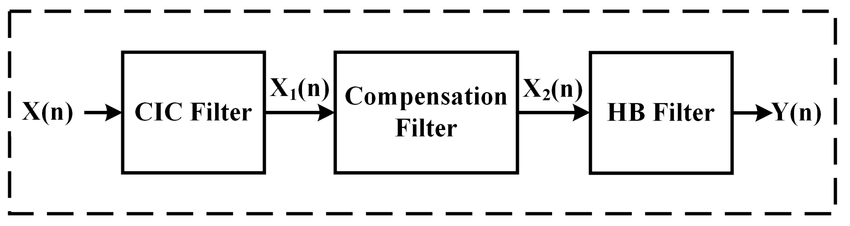
\includegraphics[width=0.8\textwidth]{Block-diagram-of-the-digital-decimation-filter.png}
    \caption{Block Diagram of the Three-Stage Digital Decimation Filter}
    \label{fig:dec_filter}
\end{figure}

Our Verilog implementation wraps the entire chain inside a top-level module (\texttt{adc\_decimation\_chain}) utilizing a shared system clock and modular handshaking via \texttt{valid}/\texttt{ready} signals to govern the multi-rate data flow.

\subsubsection{Stage 1: CIC Decimation Filter}
The CIC decimation filter is an important part of the digital decimation filter, primarily used for signal recovery, anti-aliasing, and de-sampling. Because the CIC decimation filter has the characteristics of all-tap coefficients being 1, it requires no multipliers, effectively simplifying RTL level design and saving hardware resources and area.

For the filter order, it is necessary to refer to the order of the modulator structure. The relationship between the order of the CIC decimation filter ($N$) and the order of the modulator ($L$) is $N \ge L+1$. 

\begin{figure}[H]
    \centering
    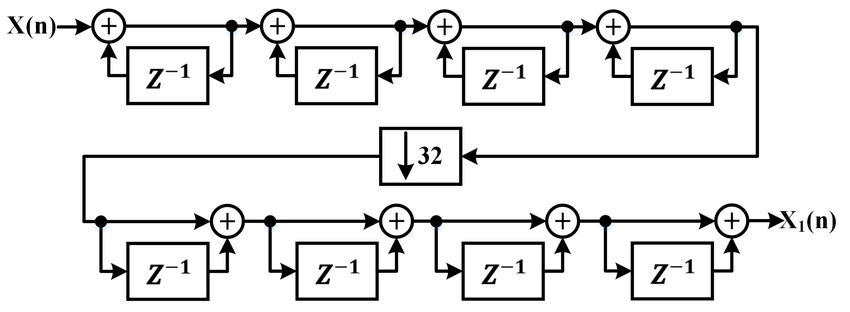
\includegraphics[width=0.8\textwidth]{Structure-of-the-CIC-decimation-filter.png}
    \caption{Structure of the CIC Decimation Filter}
    \label{fig:cic_structure}
\end{figure}

While a minimum order of 4 is standard for a 3rd-order modulator, our implementation employs an aggressive $N=10$ stage recursive structure with a decimation ratio of $R=100$. 

\textbf{Implementation Details:} To handle the massive bit growth inherent in 10 integrator stages, the internal data path of our \texttt{cic} module expands to 128 bits ($OW = 128$). To interface with the subsequent FIR stage, we designed a dedicated \texttt{cic\_scaler} and \texttt{saturate} module. The scaler adds a rounding offset before executing an arithmetic right shift of 40 bits ($128$-bit internal down to a manageable precision). The saturator then securely clamps this value to a signed 32-bit width (\texttt{FIR\_W = 32}) to prevent roll-over anomalies during extreme signal swings.

\subsubsection{Stage 2: Compensation FIR Filter}
While the CIC filter has a very good filtering effect with minimized delay units and adder units, it causes attenuation of the signal in the passband (passband roll off). Simulation of typical CIC characteristics shows passband ripple attenuation of about 1 dB, which fails stringent design requirements.

To offset this, a compensation filter is required whose frequency response characteristics are reciprocal to the CIC filter's frequency response. The required amplitude-frequency response can be expressed by an inverse sine function:
\begin{equation}
    |H_{comp}(f)| = \left| \frac{\frac{\pi f}{R}}{\sin\left(\frac{\pi f}{R}\right)} \right|^N
\end{equation}
where $R$ is the decimation factor and $N$ is the filter order. 

\begin{figure}[H]
    \centering
    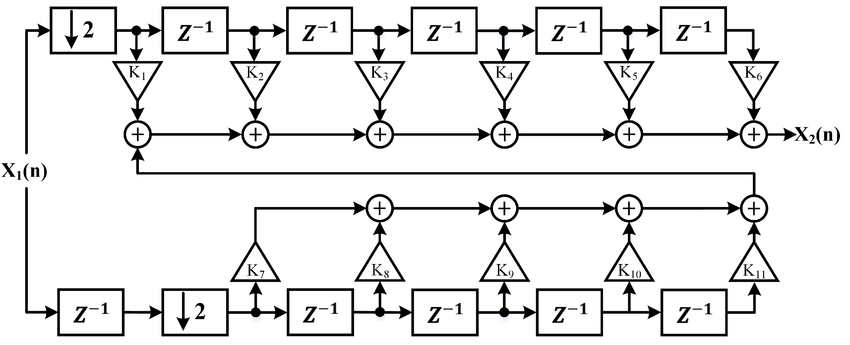
\includegraphics[width=0.8\textwidth]{Structure-of-the-multiphase-compensation-filter.png}
    \caption{Structure of the Multiphase Compensation Filter}
    \label{fig:comp_structure}
\end{figure}

\textbf{Implementation Details:} We implemented this as a 15-tap FIR filter utilizing Q15 fixed-point arithmetic. To optimize logical resource utilization, we exploited coefficient symmetry. Within the \texttt{comp\_fir} Verilog module, the 15-element delay line is paired off symmetrically (e.g., $s_0 = delay[0] + delay[14]$) before multiplying with the shared coefficients. This cuts the required DSP multiplier instances in half (from 15 down to 8). The final 48-bit accumulator output is then shifted right by 15 (with $+ (1 \ll 14)$ rounding applied) to cleanly return a 32-bit output.

\subsubsection{Stage 3: Half-Band FIR Filter}
The half-band filter is a special FIR filter characterized by a flat passband, zero odd coefficients, and a good anti-aliasing effect. These characteristics reduce hardware resources, power consumption, and area. Therefore, the last stage filter of the decimation filter utilizes the half-band filter, operating in a polyphase structure.

\begin{figure}[H]
    \centering
    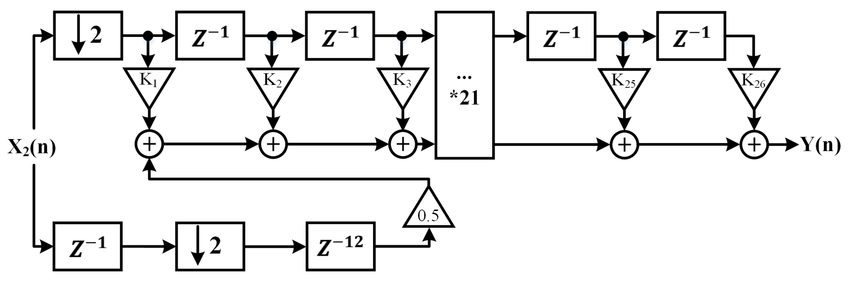
\includegraphics[width=0.8\textwidth]{Structure-of-the-multiphase-half-band-filter.png}
    \caption{Structure of the Multiphase Half-Band Filter}
    \label{fig:hb_structure}
\end{figure}

The center position unit of the half-band filter has a coefficient of 0.5, and is single extracted to form an independent branch. This specific structure reduces the multiplier unit and memory unit by about 13\%, thus reducing power consumption.

\textbf{Implementation Details:} Our \texttt{halfband\_fir} module executes a final decimation by 2. It utilizes a 7-tap delay line. Rather than instantiating a multiplier for the center tap ($h=0.5$), the design simply performs an arithmetic right shift by 1 (\texttt{center\_tap = delay\_line[3] >>> 1}). The decimation is handled efficiently via a hardware toggle (\texttt{decimation\_toggle \textasciitilde{}decimation\_toggle}) that dictates whether the \texttt{o\_valid} flag goes high, elegantly dropping every other sample without additional clock domains.

\section{Simulation and Verification of Non-Idealities}
To thoroughly test the noise immunity of the architecture, we developed a Python/Cocotb testbench that simulates real-world analog non-idealities from the upstream ADC. The base test inputs a 20Hz signal infused with:
\begin{itemize}
    \item \textbf{Clock Jitter:} $\sigma = 0.00001$ applied to the time vector.
    \item \textbf{Analog Noise:} Additive Gaussian noise with $\sigma = 0.05$.
    \item \textbf{Comparator Glitches:} Random bit flips in the PWM stream (1\% probability).
    \item \textbf{Signal Dropouts:} Held previous values mimicking lost samples (0.5\% probability).
\end{itemize}

\begin{figure}[H]
    \centering
    
\includegraphics[width=0.9\textwidth]{decimation_stages.png}
    \caption{Time-Domain Output of Decimation Stages for $f = 20$Hz}
    \label{fig:time_domain}
\end{figure}

\begin{figure}[H]
    \centering
    
\includegraphics[width=0.9\textwidth]{frequency_stages.png}
    \caption{Frequency Spectra Across the Decimation Chain}
    \label{fig:freq_domain}
\end{figure}

\subsection{Detailed Noise Impact and Mitigation}
To understand the finer details of how non-idealities affect our system, we first analyze the filter's response under a moderate noise profile. 

In a physical Sigma-Delta modulator, clock jitter translates into phase noise, while thermal analog noise and comparator glitches manifest as erroneous bit flips in the high-speed 1-bit digital stream. In the frequency domain, these non-idealities effectively raise the broadband quantization noise floor. If left unfiltered, this directly degrades the overall Equivalent Number of Bits (ENOB).

\begin{figure}[H]
    \centering
    
\includegraphics[width=0.9\textwidth]{low_noise_detail.png}
    \caption{Time-Domain Details Demonstrating Filter Smoothing under Moderate Noise}
    \label{fig:low_noise_detail}
\end{figure}

Our architecture drastically reduces the influence of this noise through aggressive low-pass filtering distributed across the three stages. The first-stage CIC filter acts similarly to a massive moving average; it effectively absorbs isolated comparator glitches and smooths out high-frequency toggling errors. The subsequent FIR compensation and half-band filters provide sharp transition bands to completely truncate the remaining out-of-band noise. Because the analog noise energy is spread over the wide 20kHz oversampled band, decimating the signal down to 100Hz naturally discards the vast majority of this noise power. 

Through our testbench simulations, our digital decimation filter effectively suppresses these artifacts, achieving an \textbf{average SNR of approximately 115.4 dB} under typical non-ideal conditions. This demonstrates excellent noise immunity and comfortably meets the stringent requirements for high-resolution ADC applications.

\subsection{High-Noise Stress Test}
To further demonstrate the aggressive filtering capabilities, an additional stress test was performed with noise dialed up significantly at the 20Hz base frequency. The non-idealities were increased to:
\begin{itemize}
    \item \textbf{Clock Jitter:} Introduced with $\sigma = 0.0001$.
    \item \textbf{Analog Noise:} Additive white Gaussian noise with $\sigma = 0.1$.
    \item \textbf{Comparator Glitches:} Random bit flips introduced with a 10\% probability.
    \item \textbf{Signal Dropouts:} Held previous values with a 5\% probability.
\end{itemize}

\begin{figure}[H]
    \centering
    
\includegraphics[width=0.9\textwidth]{high_noise_plot.png}
    \caption{Time-Domain Output of Decimation Stages for $f = 20$Hz (High Noise Environment)}
    \label{fig:high_noise}
\end{figure}
As evident from the output plot, the multi-stage filter was able to output a smooth, consistent sinusoidal signal irrespective of the extremely high non-idealities and distortions present at the raw ADC output stage.

\section{Limitations and System Constraints}
While highly effective, this architecture carries inherent operational limits. The massive cumulative decimation factor ($R_{total} = 200$) reduces a high-speed 20kHz clock down to a 100Hz output sampling rate. Based on the Nyquist criterion, this strictly limits the maximum allowable continuous signal bandwidth to below 50Hz to prevent aliasing. Additionally, while the Q15 fixed-point rounding arithmetic prevents unbounded register growth, the cascaded truncation steps inherently introduce a small, finite floor of quantization noise into the final data output.

\section{Conclusion}
This paper successfully presents and verifies a digital decimation filter utilizing a three-stage structure for Sigma-Delta ADCs. The cascade of a CIC filter, an FIR compensation filter, and a half-band filter provides optimal noise suppression while significantly downsampling the input bitstream. By strategically exploiting coefficient symmetry, single-branch extraction for zero-valued taps, and arithmetic bit-shifting in place of dedicated multipliers, the architecture achieves the necessary mathematical precision with a dramatically reduced requirement for hardware multipliers. This results in a highly efficient design tailored for minimal layout area and a low power footprint, seamlessly maintaining data integrity even under extreme analog noise conditions.

\section*{References}
\begin{enumerate}
    \item Wan, R.; Li, Y.; Tian, C.; Yang, F.; Deng W.; Tang, S.; Wang, J.; Zhang, W. ``Design and Implementation of Sigma-Delta ADC Filter." Electronics 2022, 11, 4229. \url{https://doi.org/10.3390/electronics11244229}
\end{enumerate}

\end{document}
